\documentclass[tikz,border=10pt]{standalone}
\usepackage{tikz}
\begin{document}
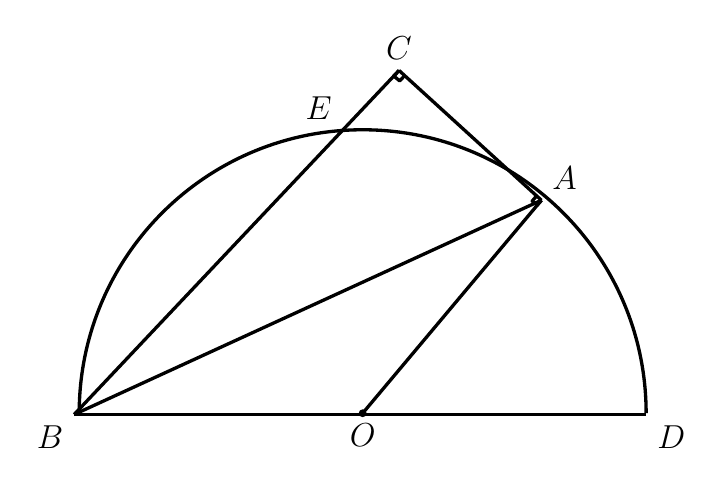
\begin{tikzpicture}[line width=1.2pt, line join=round, font=\fontsize{12.5}{15}\selectfont]
% Named points (scale s=0.014953 per px, centre (303,206), y flipped)
\coordinate (B) at (-3.634,-2.109);
\coordinate (O) at (0.030,-2.093);
\coordinate (D) at (3.634,-2.109);
% C raised by about 10 px (y +0.153), keeping ACB ~ 90 and CA tangent at A
\coordinate (C) at (0.492,2.260);
\coordinate (A) at (2.300,0.612);
% E = second intersection of line BC with the semicircle (centre O, r=3.6)
\coordinate (E) at (-0.227,1.498);
% Right-angle mark points at C (offsets kept from previous render, shifted with C)
\coordinate (C1) at (0.42500000000000,2.18950000000000);
\coordinate (C2) at (0.50000000000000,2.12750000000000);
\coordinate (C3) at (0.56650000000000,2.19800000000000);
% Right-angle mark points at A (unchanged)
\coordinate (A1) at (2.24700000000000,0.54850000000000);
\coordinate (A2) at (2.18350000000000,0.60100000000000);
\coordinate (A3) at (2.23600000000000,0.66400000000000);

% Diameter BD
\draw (B) -- (D);
% Upper semicircular arc from D to B, centred at O, radius 3.6
\draw[shift={(O)}] (3.6,0) arc (0:180:3.6);
% Segments
\draw (B) -- (C);
\draw (C) -- (A);
\draw (A) -- (B);
\draw (A) -- (O);
% Right-angle marks
\draw (C) -- (C1) -- (C2) -- (C3);
\draw (A) -- (A1) -- (A2) -- (A3);
% Centre dot
\fill (O) circle (0.05);
% Labels
\node[below left] at (B) {$B$};
\node[below] at (O) {$O$};
\node[below right] at (D) {$D$};
\node[above] at (C) {$C$};
\node[above right] at (A) {$A$};
\node[above left] at (E) {$E$};
\end{tikzpicture}
\end{document}